\chapter{Existující přístupy}

\section{Částečně pozorovatelné markovské rozhodovací procesy}

Částečně pozorovatelné markovské rozhodovací procesy (POMDP) byly úspěšně použity pro regeneraci rukou lidí po mrtvici \cite{9Pomdp} a u počítačového asistenta při mytí rukou člověkem trpícím demencí.

V obou případech byla osoba se systémem modelováno pomocí POMDP, které jsou schopné pracovat se sekvenčními dynamickými systémy, ve kterých jsou některé stavy preferované před jinými a ne vše související s procesem je plně pozorovatelné. V těchto případech nelze přímo pozorovat aktuální schopnosti uživatele.

V každém kroku je uložen belief state (pravděpodobnostní distribuce nad všemi stavy). Policy (politika) říká, kterou akci v daném kroku vybrat na základě aktuální belief state, které se na základě vybrané akce a nového pozorování aktualizuje.

\subsubsection{Influence diagramy}

Obecná POMDP mohou být řešena více exaktními způsoby, ale nejsou řešitelná s dostatečně krátkou odezvou pro naše využití. POMDP pro popsané úlohy může být redukováno na influence diagramy, které jsou snáze řešitelné.
 
Obecný influence diagram pro adaptivní systém si lze prohlédnout na Obr.~\ref{fig:ch3pomdp}. Apostrofované proměnné představují odpovídající neapostrofované proměnné v následujícím stavu. Např. hodnota napětí v následujícím stavu závisí pouze na hodnotách schopnosti a provedené akce z předchozího stavu.

\begin{figure}
  \centering
  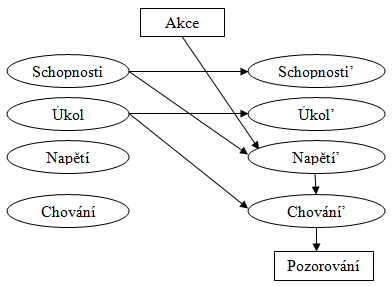
\includegraphics[width=0.5\textwidth]{ch3pomdp}
	\caption{Influence diagram pro adaptivní systémy}
	\label{fig:ch3pomdp}
\end{figure}

V každém kroku se provede právě jedna akce. Stav je popsán proměnnými 4 kategorií. Proměnná schopnosti(ability) je odhadem aktuálních schopností uživatele. Proměnná úkol(task) popisuje aktuálně prováděný úkol osobou. Proměnná napětí(stretch) znázorňuje náročnost aplikace vzhledem k aktuálnímu uživateli. Popisuje rozdíl úrovně obtížnosti zvolené akce a úrovně schopností jedince. Ideálně jsou úrovně shodné, napětí je nulové. Pokud je napětí vysoké, úkol je příliš obtížný. Jestliže je napětí záporné, úkol je příliš snadný. Proměnná chování(behavior) je přímo pozorovatelná. U pomocníka při mytí rukou je jím pozice rukou (ve vodě, na kohoutku atd.) a stav puštění vody.

\subsubsection{Příklad popisu stavu hry}

Pro lepší pochopení skupin proměnných a jejich významu uvedu příklady proměnných uvedených v článku \cite{9Pomdp}, rehabilitace po mozkové mrtvici.

Schopností je rychlost učení, jak rychle se každý uzdravuje. Úkol popisuje vektor n(r), kde pro jednotlivé hodnoty odporu ovladače je uložena maximální vzdálenost, kterou je osoba schopna dosáhnout. Napětí zde má zachován svůj význam z obecného popisu. Chování je zde nahrazeno celkovou únavou, která souvisí s následujícími pozorovanými veličinami. TTT, čas potřebný k dosáhnutí na cíl, CTRL, reprezentuje, jestli bylo cvičení vykonáno s pomocí kontroly, COMP, jestli si osoba snažila pomáhat vrchní polovinou těla místo využívání pouze její paže.

Konkrétní influence diagram můžeme vyřešit např. pomocí algoritmu PERSEUS, který najde v dostatečně krátkém čase přibližné řešení. Na základě pozorování a provedených akcí dokáže odhadnout schopnosti uživatele a vzhledem k tomu připravit odpovídající následující úlohu.

\section{Monte-Carlo prohledávání stromu}

Autoři z Pekingské univerzity vyzkoušeli spojení Monte-Carlo Tree Search(MCTS) algoritmu s dnes populárními neuronovými sítěmi. \cite{18Pac1}\cite{19Pac2}

V článcích upozorňují na nevýhodu tradičních metod DDA, kdy se obtížnost uměle mění např. přidáváním dalších a silnějších nepřátele, ale jejich inteligence zůstává stejná. Hráč se v takovém případě může cítit podveden. V Pekingu se vydali cestou dynamického vyvažování umělé inteligence a svůj přístup aplikovali na zjednodušené verzi známé hry Pac-Man.

\subsubsection{Pravidla hry Pac-Man}

Cílem hráče hrajícího za žlutou postavu Pac-Mana je sníst všechny kuličky v bludišti a zároveň se vyhýbat nepřátelům, duchům. Pac-Man zvítězí, jestliže sní všechny kuličky, duši zvítězí, jestliže chytnou Pac-Mana. Jestliže do 55 kroků žádná z těchto událostí nenastane, hra končí remízou. Oproti původnímu Pac-Manovi jsou ve hře další úpravy.


\begin{itemize}
	\item Bludiště je zmenšeno na velikost 16x16 a neobsahuje žádné Power upy.
	\item Ve hře jsou pouze dva duši místo původních 4 a mají stejnou rychlost jako Pac-Man. Z toho vyplývá, že jeden duch nikdy nemůže sám chytit Pac-Mana, duši musí spolupracovat.
	\item Pac-Man i duši se rozhodují pouze na křižovatkách. Jejich možné akce jsou jít vpravo/vlevo/nahoru/dolů, případně u křižovatek u kraje bludiště jejich podmnožina, procházení zdí je zakázáno.
\end{itemize}

\begin{figure}
  \centering
  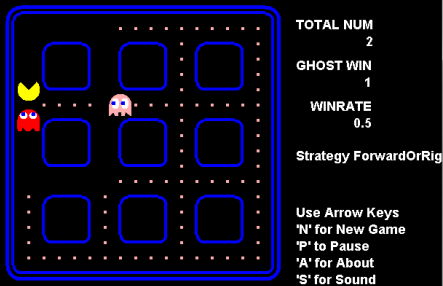
\includegraphics[width=0.5\textwidth]{ch3pacman}
	\caption{Zjednodušená verze Pac-Mana. Obrázek převzat z \cite{18Pac1}}
	\label{fig:ch3pacman}
\end{figure}

\subsubsection{Tvorba DDA pomocí MCTS}

Výkon umělé inteligence soupeřů založených na MCTS záleží na množství času, které MCTS poskytneme. Čím déle algoritmus běží, tím je pravděpodobnější inteligentnější chování duchů.

Pro účely simulace hráč Pac-Mana využíval ForwardOrRight strategii.
Pomocí opakovaných simulací s pevně daným simulačním časem získali závislost poměru vítězství (win-rate) na délce simulace. Několik získaných diskrétních hodnot proložili polynomem 4. stupně.

\begin{equation}
	y=-5,67*x^4+17,6*x^3-11,1*x^2-0,81*x+65,6
\end{equation}

V předchozí rovnici je x časem výpočtu MCTS v ms a y výsledné win-rate.
Běžný hráč chce vyhrávat přibližně v polovině případů. Vyřešením rovnice získáváme čas 105ms. Začínající hráč může upřednostnit častější vyhrávání, při win-rate 30\% (duchy) algoritmus potřebuje 28ms na výpočet.

\subsubsection{Využití neuronových sítí}
Další nevýhodou škálování AI pomocí změn simulačního času je horší využitelnost u real-time her, kde si nemůžeme dovolit věnovat stovky ms k výpočtu AI. Tento nedostatek lze odstranit využitím neuronové sítě místo MCTS.

Neuronovou síť se snažíme naučit chování odpovídající MCTS s daným simulačním časem. Při simulacích pomocí MCTS se při každém rozhodování duchů uložil stav hry, jako 23 proměnných a výsledné rozhodnutí o novém směru každého ducha.

Takto získaná data bylo použita pro učení neuronové sítě, která posléze nahradila původní algoritmus MCTS. Vstupními proměnnými byly např. pozice a směr hráče, pozice duchů a obsah sousedních dlaždic, vzdálenost mezi duchy a hráčem, čas simulace atd. Ve výstupní vrstvě bylo po 4 neuronech pro každého ducha, kde každý neuron představoval jeden zvolený směr.

Neuronové sítě odstranily časovou divergenci pro různé AI, ale naopak přinesly do systému jistou míru nepředvídatelnosti.

\section{Producent – konzument}

V mnohých hrách můžeme pozorovat vztah producent – konzument mezi světem a hráčem. Jestliže hráč získá ze světa moc prostředků, hra přestává být výzvou a naopak. Má-li hráč málo prostředku (např. munice, zdraví), může být frustrován kvůli vysoké obtížnosti.
Robin Hunicke popsala systém The Hamlet integrovaný do Half-Life SDK\cite{20Hun}, který vyvažuje obtížnost hry právě pomocí výměny zdrojů mezi světem a hráčem. Half-Life patří mezi klasické zástupce first-person shooter (FPS, „střílečky“).

\subsubsection{Použitá metrika}

Hunicke používá metriku pravděpodobnost smrti hráče. Ze série měření určí pravděpodobnostní distribuci poškození udělené hráči protivníkem během boje. Předpokládá Gaussovskou distribuci :

\begin{equation}
	   p(x)=\frac{1}{\sigma\sqrt{2\pi}}\mathrm{e}^{\frac{-(x-\mu)^2/2}{\sigma^2}}
\end{equation}

Pomocí určitého integrálu F(d) můžeme spočítat pravděpodobnost utrpění poškození menší, nebo rovnu d, kterou lze využít pro určení pravděpodobnosti přežití, jestliže má hráč aktuální zdraví rovné hodnotě d.

\begin{equation}
	   F(x) = \int_d^\infty p(x)\,\mathrm{d}x
\end{equation}

Dosazením za p(x) získáváme rovnici \ref{eq:integraldamage}.

\begin{equation} \label{eq:integraldamage}
	   F(x) = \frac{1}{\sigma\sqrt{2\pi}}\int_d^\infty \mathrm{e}^{\frac{-(x-\mu)^2/2}{\sigma^2}}\,\mathrm{d}x
\end{equation}

Tento integrál lze aproximovat funkcí erf z knihovny C++. V následujícím vzorci h odpovídá aktuálnímu zdraví hráče, 
	\(\mu, \sigma
\)
 pro střední hodnotu a standardní odchylku poškození od aktuálního oponenta v nějakém čase t v budoucnu.

\begin{equation} \label{eq:integraldamage}
	   F(d_t) = 1-\frac{1}{2}(1+erf(\frac{h-\mu t}{\sigma\sqrt{2t}}))
\end{equation}

Během souboje se zaznamenává poškození d, které každý z protivníků udělí hráči. Na základě těchto hodnot a vzorců výše lze přibližně spočítat pravděpodobnost smrti hráče.

\subsubsection{Vyvažující strategie}

Systém Hamlet mění obtížnost na základě poptávky a nabídky. Na straně nabídky může systém zasáhnout umisťováním předmětů v herním prostředí (lékárničky, munice, zbraně). Dále může přizpůsobovat účinnost a přesnost hráčových zbraních, projev brnění apod.

Na straně poptávky manipulovat s nepřáteli (změnou jejich třídy, množství, počtu jejich životů, určením místa jejich objevení se na mapě). Stejně jako u hráče lze přizpůsobit sílu a přesnost jejich zbraní.

Autoři se snaží držet hráče v tzv. „komfortní zóně“, kdy se hráč cítí relativně v bezpečí. Jestliže se v průběhu boje zvedne pravděpodobnost úmrtí nad 40\%, Hamlet začne zasahovat do hry výše uvedenými způsoby.

Cílem této politiky je udržet zdraví hráče na střední hodnotě 60 se standardní odchylkou 15 bodů. Hamlet je navržen tak, aby pomáhal hráčům, kteří mají problémy, ale na druhou stranu, aby je neprotahoval za každou cenu skrz herní úrovně.

